\chapter{Non-relativistic Quantum Field Theory}
A general non-relativistic field theory is described by the action (with repeated indices automatically summed):
\begin{equation}
\begin{aligned}
	S &= S_0 + S_{\mathrm{int}} = \int dt \int d^d x \mathcal{L}_0 - \int dt\ \mathcal{V}_{\mathrm{int}}, \\
	\mathcal{L}_0 &= \bar\psi_a(x) (i\delta_{ab}\partial_t-\hat H_{ab})\psi_b(x).
\end{aligned}
\end{equation}
where the field operator $\psi(x)$ can be bosonic or fermionic, which is denoted by a number $\zeta=\pm 1$, and $\mathcal{V}_{\mathrm{int}}$ is the interaction Lagrangian.
A general interaction has the form
\begin{equation}
	\mathcal{V}_{\mathrm{int}} = \sum_{abcd}\int \prod_{i=1}^4 d^d x_i \ \bar\psi_{c}(x_3)\bar\psi_{d}(x_4) V_{abcd}(x_1,x_2,x_3,x_4) \psi_{b}(x_2)\psi_{a}(x_1).
\end{equation}
Note that the classical equation of motion for the free field satisfies the Schr\"{o}dinger equation:
\begin{equation}
	\partial_\mu \frac{\partial \mathcal L_0}{\partial(\partial_\mu \bar\psi_a(x))} - \frac{\partial \mathcal L_0}{\partial\bar{\psi}_a(x)} 
	= - i\partial_t \psi_a(x) + \hat H_{ab}\psi_b(x) = 0.
\end{equation}

We are mostly work with finite system size $L^d$ with UV cutoff $\Lambda = \pi/a$ (where $a$ is the lattice spacing, and $L = Na$). The spatial Fourier transformation is
\begin{equation}
	\tilde{\psi}_a(k) = \int_{L^d} d^dx e^{-i k \cdot x}\psi_a(x), \quad
	\psi_a(x) = \frac{1}{L^d}\sum_{k} e^{i k \cdot x}\tilde{\psi}_a(k).
\end{equation}
For the finite size, the momentum is discretized: $k = 2\pi n_k/L$, $n_k \in \mathbb Z$.
The summation in the thermodynamic limit becomes the integral:
\begin{equation}
	\frac{1}{L^d}\sum_k \longrightarrow \int_{|k|<\Lambda} \frac{d^dk}{(2\pi)^d}.
\end{equation}
In the momentum space, the free theory can be simplified:
\begin{equation}
	S_0 = \int dt \int \frac{d^d k}{(2\pi)^d} \tilde{\bar\psi}_a(k) [i\partial_t-\varepsilon_a(k)]\tilde{\psi}_a(k).
\end{equation}
The interaction in the momentum space is described by the vertex function:
\begin{equation}
	\tilde V_{abcd}(k_1,k_2,k_3,k_4)
	= \int \prod_{i=1}^4 d^d x_i e^{i(k_1x_1+k_2x_2-k_3x_3-k_4x_4)} V_{abcd}(x_1,x_2,x_3,x_4).
\end{equation}
Because of the momentum conservation, the vertex will contain a delta function factor.

Consider the Coulomb repulsive potential $e^2/r$, in the field theory formalism, the coefficient $V_{abcd}(x_1,x_2,x_3,x_4)$ is
\begin{equation}
\begin{aligned}
	\frac{V(x_1-x_2)}{2!2!}\left[\delta_{ac}\delta_{bd}\delta^{(3)}(x_1-x_3)\delta^{(3)}(x_2-x_4) - \delta_{ad}\delta_{bc}\delta^{(3)}(x_1-x_4)\delta^{(3)}(x_2-x_3)\right],
\end{aligned}
\end{equation}
where the factor $\frac{1}{2!2!}$ is the symmetry from interchanging the fermion fields.
In momentum space:
\begin{equation}
	V_{abab}(k_1,k_2,k_3+q,k_4-q) = \frac{1}{2!2!} V_{\mathrm{Coul}}(q),
\end{equation}
where the Coulomb potential in the momentum space is
\begin{equation}
\begin{aligned}
	V_{\mathrm{Coul}}(q) 
	&=  \lim_{\alpha\rightarrow0}e^{2}\int_{0}^{\infty}dr\ 2\pi r^{2} \int_{-1}^{+1}d\left(\cos\theta\right)\frac{e^{-iqr\cos\theta-\alpha r}}{r} \\
	&=  \lim_{\alpha\rightarrow0}\frac{2\pi e^{2}}{iq}\int_{0}^{\infty}dr\left(e^{iqr-\alpha r}-e^{-iqr-\alpha r}\right)\\
 	&=  \lim_{\alpha\rightarrow0}\frac{4\pi e^{2}}{q^{2}+\alpha^{2}}
	=  \frac{4\pi e^{2}}{q^{2}}.
\end{aligned}
\end{equation}



\section{Action in Euclidean Space}

The original real-time partition function is defined as\footnote{As with the relativistic case, we introduce an auxiliary source $J$, which is bosonic/fermionic if the field $\psi$ is bosonic/fermionic.
}
\begin{equation}
	Z[J] = \int D[\bar\psi,\psi] \exp\left\{i\int dt \int d^dx \left[\mathcal{L}+\bar{J}_a(x)\psi_a(x)+\bar{\psi}_a(x)J_a(x)\right]\right\}.
\end{equation}
If we make a analytic continuation of $t$ to the complex plane:\footnote{Note that in the frequency domain, the singularities for positive frequency lies below the complex plane, as we always include an infinitesimal $-i\epsilon$ to the energy (mass) term of the theory in ensure convergence. So, the rotation of the real axis anti-clock-wisely to the imaginary axis will not cross any singularity, and thus the can be analytically extended.}
\begin{equation}
	t \rightarrow -i\tau, \quad \omega \rightarrow i\omega.
\end{equation}
In this way the free action transforms as:
\begin{equation*}
	iS_0 = i \int dt dx\ \psi(\bm x, t) (i\partial_t - E) \psi(\bm x, t) \rightarrow 
	-\int d\tau dx\ \psi(\bm x, \tau) (\partial_\tau + E) \psi(\bm x, \tau).
\end{equation*}
The partition function can then be written as:
\begin{equation}
	Z[J] = \int D[\bar\psi,\psi] e^{-S_0[\bar\psi,\psi]+\bar{J}\cdot\psi+\bar{\psi}\cdot J},
\end{equation}
where the Euclidean free action defined as:
\begin{equation}
	S = \int d\tau \left[\int d^dx\ \bar\psi_a(\bm x,\tau) (\delta_{ab}\partial_\tau+\hat H_{ab})\psi_b(\bm x,\tau) + \mathcal{V}_\mathrm{int}\right].
\end{equation}

The Euclidean action is suitable to describe the system both in zero temperature or finite temperature.
For finite temperature case, the integral over the imaginary time $\tau$ is over $[0,\beta)$.
The Fourier transformation of the field on the imaginary time domain is defined as:
\begin{equation}
	\tilde\psi(\omega_n) = \int_0^\beta d\tau e^{i\omega_n\tau} \psi(\tau),\quad
	\psi(\tau) = \frac{1}{\beta}\sum_{\omega_n} e^{-i\omega_n\tau} \tilde\psi(\omega_n).
\end{equation}
Under such convention, in the thermodynamic limit and zero-temperature limit, the spatial-temporal Fourier transformation agrees with the relativistic case (up to a Wick rotation).



\subsection{Free Field Theory}

The Fourier transformation of the free field action is
\begin{equation}
	S_0 = \frac{1}{\beta}\sum_{\omega_n} \int_{\Lambda} \frac{d^dk}{(2\pi)^d}
	\tilde{\bar{\psi}}_a(k,\omega_n)\left[-i\omega_n + \tilde{H}_{ab}(k)\right]\tilde{\psi}_b(k,\omega_n).
\end{equation}
The partition function with source is
\begin{equation}
	\frac{Z_0[J]}{Z_0[0]} = \exp\left[-\frac{1}{\beta}\sum_{\omega_n} \int_{\Lambda} \frac{d^dk}{(2\pi)^d}\tilde{\bar J}_a(k,\omega_n) \tilde{G}_{ab}(k,\omega_n) \tilde{J}_b(k,\omega_n) \right],
\end{equation}
where the Green's function is
\begin{equation}
	\tilde{G}_{ab}(k,\omega_n) = \left[\frac{1}{i\omega_n - \tilde{H}(k)}\right]_{ab}.
\end{equation}

Unlike the relativistic case, the value of the value of partition function without source $Z_0[0]$ is related to the free energy.
We can express it formally as
\begin{equation*}
	Z_0[0]= \left[\det (-G_{ab})^{-1}\right]^{-\zeta}.
\end{equation*}
To get the correct dimensionality, we set the determinant as
\begin{equation*}
	Z_0[0] \equiv \prod_{k,\omega_n}\left\{\beta \det\left[-i\omega_n+\tilde{H}(k)\right]\right\}^{-\zeta}.
\end{equation*}
Thus the free energy is
\begin{equation}
	F = -\frac{1}{\beta} \ln Z_0
	= \zeta \sum_{k,\omega_n} \ln\left\{\beta\det\left[-i\omega_n+\tilde{H}(k)\right]\right\}.
\end{equation}


\subsection{Matsubara Summation}
Now consider the summation on Matsubara frequency:
\begin{equation}
	\sum_{\omega_n} f(\omega_n) = 
	\begin{cases}
		\sum_n f(\frac{2n\pi}{\beta}) & \mathrm{bosonic} \\
		\sum_n f(\frac{(2n+1)\pi}{\beta}) & \mathrm{fermionic}
	\end{cases}.
\end{equation}
The frequency is capture by the singularities of the density function of the states:
\begin{equation}
	\rho(z) = \begin{cases}
		\frac{1}{\exp(\beta z)-1} & \mathrm{bosonic} \\
		\frac{1}{\exp(\beta z)+1} & \mathrm{fermionic}
	\end{cases}.
\end{equation}
The residue on imaginary frequency $i\omega_n$ is alway $\frac{1}{\beta}$. In this way, the summation is:
\begin{equation}
	\frac{1}{\beta}\sum_{\omega_n} f(i\omega_n) 
	= \frac{1}{2\pi i} \oint \rho(z)f(z)
	= -\sum_{k} \mathrm{Res}\ \rho(z)f(z)|_{z=z_k}.
\end{equation}

\subsubsection*{Summation of Green's function}
Consider the frequency summation for the correlation function:
\begin{equation}
	\frac{1}{\beta}\sum_{\omega_n} \tilde{G}_0(k) 
	= \frac{1}{\beta}\sum_{\omega_n}\frac{1}{i\omega_n-E_{p}}
	= -\mathrm{Res} \left. \frac{\rho(z)}{z-E_{p}}\right|_{z=E_{p}}
	= \rho(E_{p}).
\end{equation}


\subsubsection*{Summation of Green's function}
Consider the frequency summation for the correlation function:
\begin{equation}
	\sum_{\omega_n} \langle\bar\psi_{\vec p,\omega_n}\psi_{\vec p, \omega_n}\rangle = \frac{1}{\beta}\sum_{\omega_n}\frac{1}{-i\omega_n+\epsilon_{\vec p}}
	= \mathrm{Res} \left. \frac{\rho(z)}{z-\epsilon_{\vec p}}\right|_{z-\epsilon_{\vec p}}
	= \rho(\epsilon_{\vec p}).
\end{equation}

\subsubsection*{Free Energy Summation}
Consider the free energy
\begin{equation}
	F = -\frac{1}{\beta}\ln Z 
	= -\frac{1}{\beta}\sum_{\omega_n}\ln[\beta(-i\omega_n+E_{\vec p})]
	= \frac{1}{2\pi i} \oint dz \rho(z)\ln[\beta(\xi - z)].
\end{equation}
To calculate the summation, we consider the line integral along the loop:
\begin{equation*}
	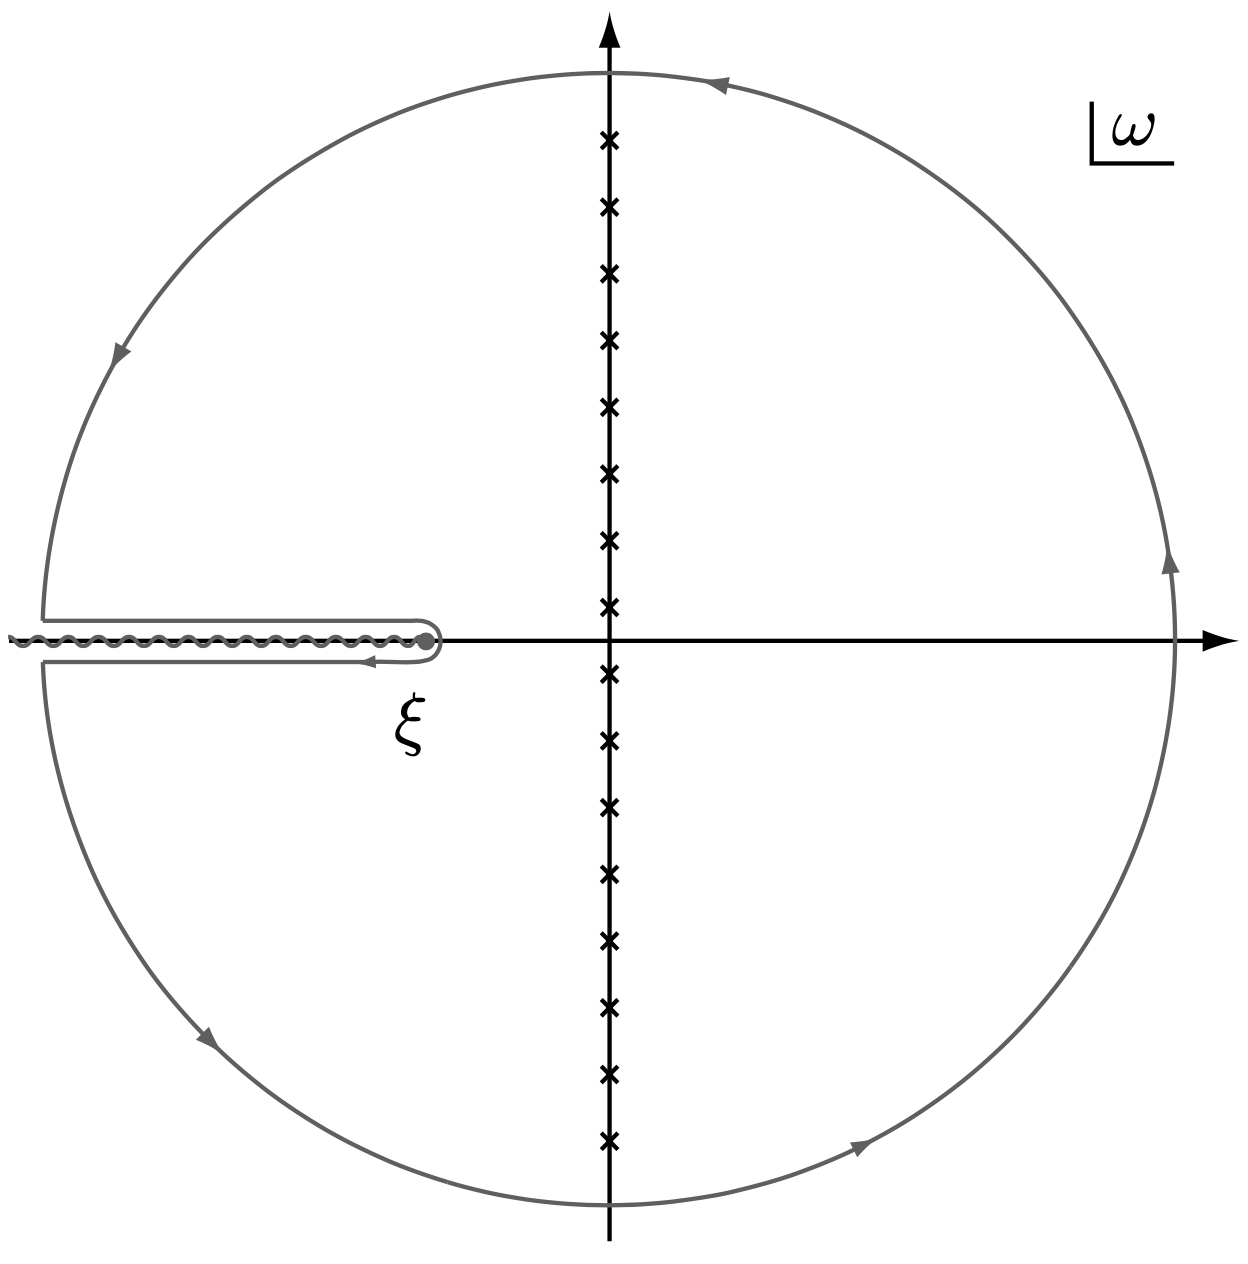
\includegraphics[width=0.25\linewidth]{pics/FqSum.png}
\end{equation*}
The free energy is
\begin{equation}
\begin{aligned}
	F &= \frac{1}{2\pi i}\int_{-\infty}^\infty dx \rho(x)\ln\left(\frac{\xi-x-i\epsilon}{\xi-x+i\epsilon}\right) \\
	&= \frac{-\zeta}{2\pi i\beta} \int_{-\infty}^{\infty}dx \ln(1-\zeta e^{-\beta z})\left(\frac{1}{x+i\epsilon-\xi}-\frac{1}{x-i\epsilon-\xi}\right),
\end{aligned}
\end{equation}
where we integrate the expression by part, noticing that
\begin{equation}
	\frac{d}{dz} \frac{\zeta}{\beta} \ln(1-\zeta e^{-\beta z}) = \frac{1}{e^{\beta z}-\zeta} = \rho(z)
\end{equation}
Using the identity
\begin{equation*}
	\lim_{\epsilon\rightarrow 0^+} \frac{1}{x+i\epsilon} = -i\pi\delta(x) + \mathcal{P}\frac{1}{x},
\end{equation*}
the above expression can be simplified to
\begin{equation}
	F = \frac{\zeta}{\beta} \ln(1-\zeta e^{-\beta\zeta}).
\end{equation}


\section{Fermi Liquid Theory}
In this section, we are considering the system of weakly interacting Fermi gas.
To be specific, we consider the lattice Hamiltonian:
\begin{equation}\label{eq:FL-gen-ham}
	H = -\frac{1}{2}\sum_{\langle i,j \rangle} (c_i^\dagger c_{j} + c_{j}^\dagger c_i) + \mu\sum_i c_i^\dagger c_i + \sum_{i,j,k,l} u_{ijkl} c_i^\dagger c_j^\dagger c_k c_l.
\end{equation}
In the following, we investigate the effective field theory near the Fermi surface.
We discuss the RG flow of the couplings (mainly for two dimensional system).
Then we carry out the perturbative calculation for the correlation functions. 

\subsection{Effective Field Theory for Interacting Fermi Systems}
The low-energy manifold is an annulus of thickness $2 \Lambda$ symmetrically situated with respect to the Fermi circle $K=K_{\mathrm{F}}$.
The dispersion for the free lattice model is
\begin{equation}
	E(\bm K) = -\cos K_x - \cos K_y \simeq -2 + \frac{\bm K^2}{2}.
\end{equation}
For a given chemical potential $\mu$, the Fermi circle is $K_F = \sqrt{2m\mu}$, we can linearize the dispersion near the Fermi surface:
\begin{equation}
	E(\bm K) = \frac{\bm K^2-K_F^2}{2m} \simeq \frac{K_F}{m}k \equiv v_F k, \quad
	k\equiv |K|-K_F
\end{equation}
The partition function is:
\begin{equation}
	Z_0 = \sum_\theta \sum_{|k|<\Lambda}\int D\left[\bar\psi(k,\theta,\omega),\psi(k,\theta,\omega)\right] e^{-S_0},
\end{equation}
where the free field action is:\footnote{A factor of $K_{\mathrm{F}}$ has been absorbed in the field.}
\begin{equation}
	S_0 = \int \frac{d\theta}{2\pi} \int^\Lambda_{-\Lambda}\frac{dk}{2\pi} \int^\infty_{-\infty}\frac{d\omega}{2\pi} \bar\psi(k,\theta,\omega)(-i\omega+v_F k)\psi(k,\theta,\omega).
\end{equation}
Consider the quartic interaction
\begin{equation}
	\delta S_4 = \frac{1}{4}\int_{\bm K,\theta,\omega} \bar\psi(4)\bar\psi(3)\psi(2)\psi(1)u(4,3,2,1)
\end{equation}
where we eliminate one of the four sets of variables, say, the one numbered 4, by integrating them against the delta functions:
\begin{equation}
	\int_{K,\theta,\omega}
	=\prod_{i=1}^{3} \int_{0}^{2 \pi} \frac{d \theta_{i}}{2 \pi} \int_{-\Lambda}^{\Lambda} \frac{d k_{i}}{2 \pi} \int_{-\infty}^{\infty} \frac{d \omega_{i}}{2 \pi} \theta\left(\Lambda-\left|k_{4}\right|\right), \quad 
	k_4 = |\bm K_4|-K_F.
\end{equation}
The $\omega$ integral is easy: since all $\omega$'s are allowed, the condition $\omega_4=\omega_1+\omega_2-\omega_3$ is always satisfied for any choice of the first three frequencies. 
The same would be true for the momenta if all momenta were allowed. 
But they are not; they are required to lie within the annulus of thickness $2\Lambda$ around the Fermi circle. 
Consequently, if one freely chooses the first three momenta from the annulus, the fourth could have a length as large as $3K_F$. 
The role of $\delta(\Lambda-|k_4|)$ is to prevent exactly this.

\subsubsection*{Momentum Constraint}
Note that $k_4$ can be expressed as
\begin{equation}
	k_4 = |(K_F+k_1)\bm \Omega_1+(K_f+k_2)\bm \Omega_2-(K_F+k_3)\bm \Omega_3|-K_F.
\end{equation}
When doing RG towards the Fermi surface, the integral measure will not preserve the preserve the original form.
The situation is clearly is we use a smooth cutoff
\begin{equation}
	\theta(\Lambda-|k_4|) \rightarrow e^{-|k_4|/\Lambda},
\end{equation}
and define $\Delta\equiv \bm \Omega_1+\bm \Omega_2-\bm \Omega_3$, $k_4$ in this way behaves as
\begin{equation}
	k_4 = (|\Delta|-1)K_F + O(k).
\end{equation}
The integral then change to:
\begin{equation}
\begin{aligned}
	& \prod_{i=1}^{3} \int_{-\Lambda}^{\Lambda} \frac{d k_{i}}{2\pi} 
		\int \frac{d \theta_{i}}{2 \pi} \int \frac{d \omega_{i}}{2 \pi} 
		e^{-||\Delta|-1|\frac{K_F}{\Lambda}} u(k,\theta,\omega) 
		\bar\psi \bar\psi \psi \psi \\
	\overset{\mathrm{RG}}{\longrightarrow} & \prod_{1}^{3} \int_{-\Lambda}^{\Lambda}
		\frac{d k_{i}^{\prime}}{2 \pi} 
		\int \frac{d \theta_{i}}{2 \pi} 
		\int \frac{d \omega_{i}^{\prime}}{2 \pi} 
		e^{-|| \Delta|-1|\frac{sK_F}{\Lambda}} 
		u\left(\frac{k^{\prime}}{s} \frac{\omega^{\prime}}{s} \theta\right) 
		\bar\psi \bar\psi \psi \psi.
\end{aligned}
\end{equation}
We can then get the RG transformation of $u$ as
\begin{equation}
	u'(k',\theta,\omega') = e^{-||\Delta|-1|\frac{(s-1)K_F}{\Lambda}}u\left(\frac{k'}{s},\theta,\frac{\omega'}{s}\right).
\end{equation}
By Taylor expansion, we conclude that the only couplings that survive the RG transformation without any decay correspond to the cases in which $|\Delta|=1$, and without momentum dependence.

\begin{figure}[]
	\centering
	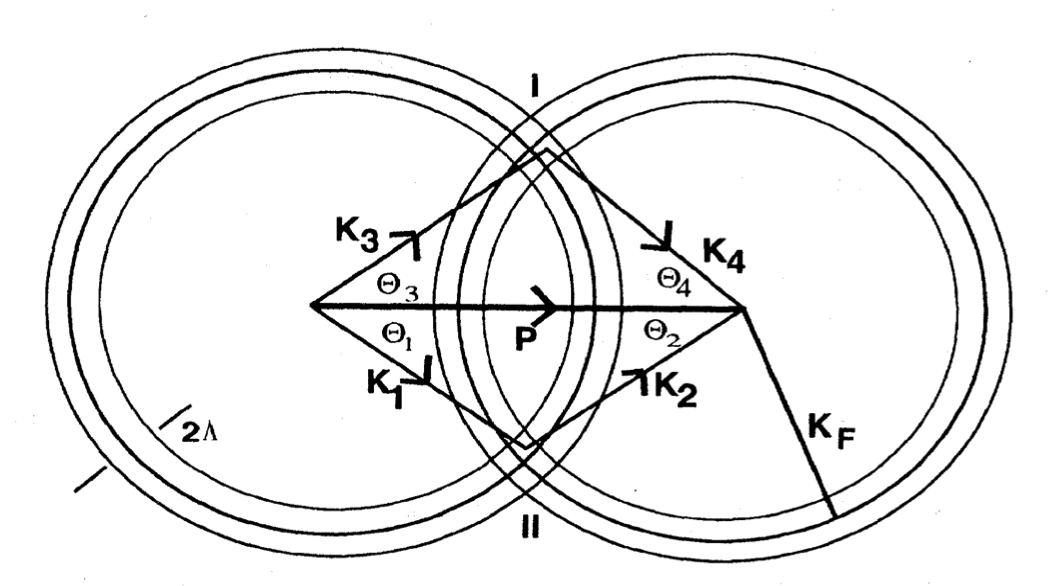
\includegraphics[width=0.5\linewidth]{pics/FL-kcons.png}
	\caption{The geometric construction for determining the allowed values of momenta. If $K_{1}$ and $K_{2}$ add up to $P$, then $K_{3}$ and $K_{4}$ are constrained as shown, if they are to add up to $P$ and lie within the cutoff. If the incoming momenta $K_{1}$ and $K_{2}$ are equal and opposite, the two shells coalesce and $K_{3}$ and $K_{4}$ are free to point in all directions, as long as they are equal and opposite.}
	\label{fig:FL-kcons}
\end{figure}

This equation has only three solutions (see also Fig.~\ref{fig:FL-kcons}):
\begin{equation}
\begin{aligned}
	&\text{Case I:} \quad \bm \Omega_1 = \bm \Omega_3, \\
	&\text{Case II:} \quad \bm \Omega_2 = \bm \Omega_3, \\
	&\text{Case III:} \quad \bm \Omega_1 = -\bm \Omega_2.
\end{aligned}
\end{equation}
Because of the rotational symmetry, the marginal vertex functions are determined solely by two functions:
\begin{eqnarray}
	u[\theta_1,\theta_2,\theta_1,\theta_2] &\equiv& F(\theta_1,\theta_2) = F(\theta_1-\theta_2), \\
	u[\theta_1,\theta_2,\theta_2,\theta_1] &=& -F(\theta_1-\theta_2), \\
	u[\theta_1,-\theta_1,\theta_3,-\theta_3] &\equiv& V(\theta_1,\theta_3) = V(\theta_1-\theta_3).
\end{eqnarray}
Note that the manifestation of the Pauli principle on $F$ and $V$ is somewhat subtle: $F$ will not be antisymmetric under $1 \leftrightarrow 2$ since, according to the way it is defined above, we cannot exchange 1 and 2 without exchanging 3 and 4 at the same time. 
On the other hand, since 3 and 4 can be exchanged without touching 1 and 2 in the definition of $V$, $V$ must go to $-V$ when $1 \leftrightarrow 3$.

\subsection{One-loop RG for 2D System}
We first consider the loop correction to the chemical potential:
\begin{equation}
\begin{aligned}
	\mu^{(2)}(k,\theta,\omega) 
	&= \int_{d\Lambda}\frac{dK'}{2\pi} \int \frac{d\omega'}{2\pi} \int \frac{d\theta'}{2\pi} \frac{F(\theta-\theta')}{i\omega-v_F k'} \\
	&= \int_{-\Lambda}^{-\Lambda+\Lambda dt}\frac{dK'}{2\pi} \int \frac{d\theta'}{2\pi} F(\theta-\theta') \\
	&= \frac{\Lambda}{2\pi} \left[\int\frac{d\phi}{2\pi} F(\phi)\right] dt.
\end{aligned}
\end{equation}
For the vertex correction, again we should consider three channels corresponding to the diagrams:
\begin{equation}
	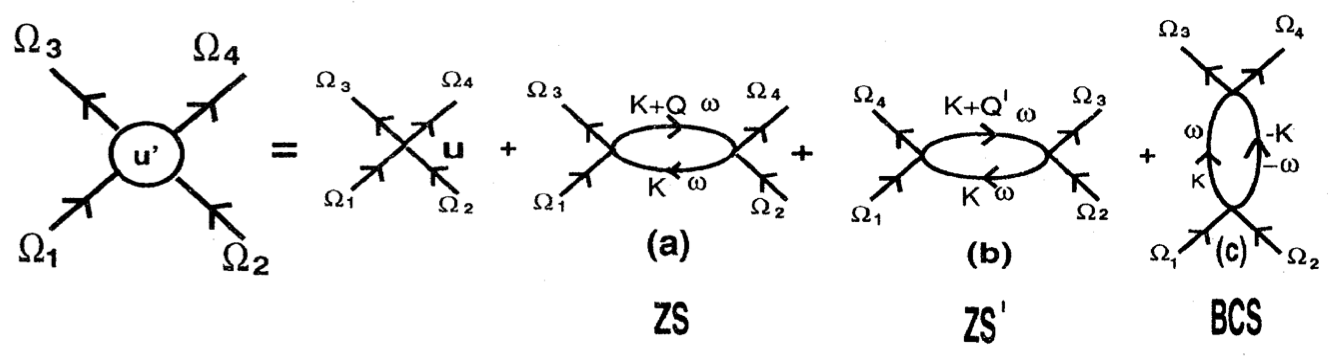
\includegraphics[align=c, width=0.7\linewidth]{pics/FL-4.png}
\end{equation}
First we consider the correction to the $F(\theta)$.
The contribution from the ZS channel (the momentum transfer $Q \simeq 0$) is
\begin{equation}
	F^{(2)}_{\mathrm{ZS}}(\theta_1-\theta_2) = \int_{d\Lambda}\frac{dk}{2\pi}\int \frac{d\omega}{2\pi} \int \frac{d\theta}{2\pi} \frac{F(\theta_1-\theta)F(\theta-\theta_2)}{(i\omega-v_F k)^2}.
\end{equation}
Since two poles of the integrant lie at the same half plane, we can alway choose to close the loop integral along the other half, and thus getting zero contribution.

\begin{figure}[]
	\centering
	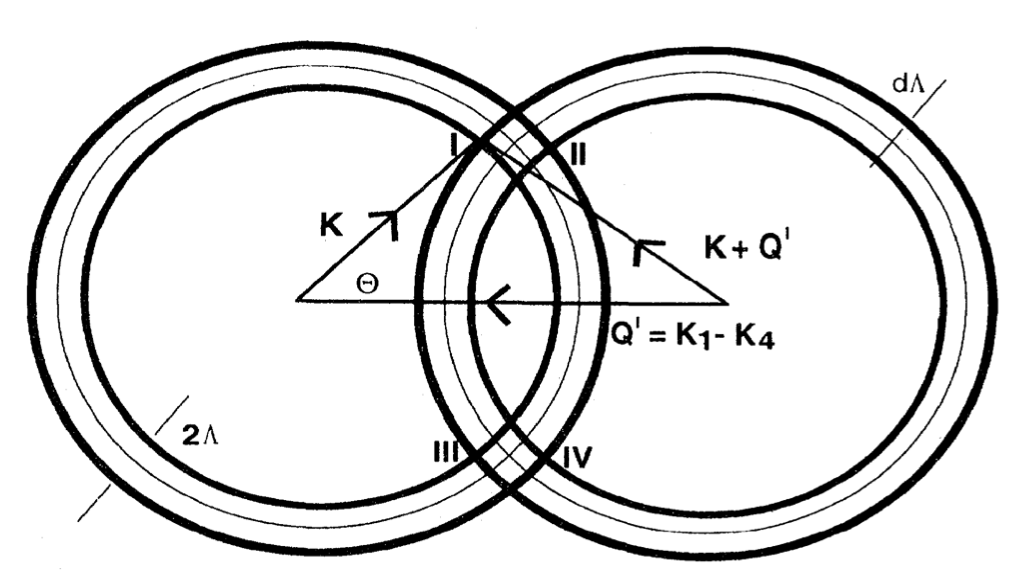
\includegraphics[width=0.4\linewidth]{pics/FL-kshell.png}
	\caption{Construction for determining the allowed values of loop momenta in ZS'. The requirement that the loop momenta come from the shell and differ by $Q'$ forces them to lie in one of the eight intersection regions of width $d\Lambda^2$.}
	\label{fig:FL-kshell}
\end{figure}

For the ZS' channels, the momentum conservation condition (see Fig.~\ref{fig:FL-kshell}) restrict the phase space to be of order $d\Lambda^2$, and thus has no relevant contribution to $F(\theta)$.
Finally, for the same kinematical reason, the BCS diagram does not renormalize $F(\theta)$ at one loop.
Consider Fig.~\ref{fig:FL-kcons}, with $K_3$ and $K_4$ replaced by the two momenta in the BCS loop, $K$ and $P-K$.
In each annulus we keep just two shells of thickness $d\Lambda$ at the cutoff corresponding to the modes to be eliminated. 
The requirement that $K$ and $P-K$ lie in these shells and also add up to $P$ forces them into intersection regions of order $d\Lambda^2$. 
This means the diagram is just as ineffective as the ZS' diagram in causing a flow. 
Thus any $F$ is a fixed point to this order.

Now we consider the correction to the $V(\theta)$ function.
We choose the external momenta equal and opposite and on the Fermi surface. 
The ZS and ZS' diagrams do not contribute to any marginal flow for the same reason that BCS and ZS' did not contribute to the flow of $F(\theta)$.
But the BCS diagram produces a flow:
\begin{equation}
\begin{aligned}
	V^{(2)}_{\mathrm{BCS}}(\theta_1-\theta_3) 
	&= -\frac{1}{2}\int_{d\Lambda}\frac{dk}{2\pi}\int\frac{d\omega}{2\pi}\int\frac{d\theta}{2\pi} 
		\frac{V(\theta_1-\theta)V(\theta-\theta_3)}{(i\omega-v_F k)(-i\omega-v_F k)} \\
	&= -\frac{dt}{4\pi v_F}\int \frac{d\theta}{2\pi}V(\theta_1-\theta)V(\theta-\theta_3).
\end{aligned}
\end{equation} 
We can simplify the picture by going to angular momentum eigenfunctions,
\begin{equation}
	V(\theta) = \sum_l e^{il\theta} V_l,
\end{equation}
which gives the RG flow as
\begin{equation}
	\frac{dV_l}{dt} = -\frac{V_l^2}{4\pi v_F}.
\end{equation}
The solution to the RG flow is:
\begin{equation}
	V_l(t) = \frac{V_l(0)}{1+\frac{V_l(0)}{4\pi v_F}t}.
\end{equation}
What these equations tell us is that if the potential in angular momentum channel $l$ is repulsive, it will get renormalized (logarithmically) down to zero, while if it is attractive, it will run off to large negative values signaling the BCS instability. 
This is the reason the $V$'s are excluded in Landau theory, which assumes we have no phase transitions.\footnote{Remember that the sign of any given $V_l$ is not necessarily equal to that of the microscopic interaction. Kohn and Luttinger have shown (PRL, 15, 524 (1965)) that some of them will be always negative. Thus, the BCS instability is inevitable, though possibly at absurdly low temperatures or absurdly high angular momentum $l$.}



